
\section{Arquitectura de la solución}
En este apartado continuaremos profundizando en los detalles de la solución propuesta en el apartado \ref{solucion}. Describiremos tanto la arquitectura de la aplicación generadora del código como de la aplicación esqueleto de Android que instanciaremos con la plantilla de un informe DICOM-SR.\par

\subsection{Aplicación Android}
Nuestro objetivo último es disponer de una aplicación Android para una determinada ontología de informe médico,  que facilite al personal clínico la tarea de rellenar los informes de los pacientes siguiendo el estándar DICOM-SR. Por lo tanto el código que generaremos deberá contener todos los componentes de una aplicación Android.

\subsubsection{Justificación para desarrollar un aplicación nativa para Android}

En este proyecto generamos una aplicación nativa para Android. Antes de entrar en profundidad a describir la anatomía de una aplicación Android, dedicaremos unas líneas a justificar la decisión de escribir una aplicación nativa para Android en lugar de desarrollar una aplicación genérica en HTML5, o utilizando frameworks como Phonegap \cite{phonegap}, Titanium \cite{titanium} o Corona \cite{corona} para crear una aplicación híbrida, o ya que nuestro generador de código está escrito en Python porque no utilizar Python también en Android mediante el framework Kivy\cite{kivy}.\medskip\par

Comenzaremos por argumentar esta última opción ya que es también la más sencilla de rebatir. Que escribamos el generador de código en un lenguaje no implica que el software generado deba estar escrito en ese mismo lenguaje, de hecho esta disociación es un punto fuerte de la generación de código, como ya explicamos en el apartado \ref{sec:generacion-codigo}.\par 
La utilización de Kivy está justificada cuando queremos hacer una aplicación multiplataforma, para dispositivo móviles y de escritorio, sin necesidad de reescribir del código. Aporta la potencia y simplicidad de Python y está recomendado para el desarrollo de juegos o aplicaciones con gran carga gráfica, ya que en el caso de aplicaciones genéricas la interfaz que crea este framework no es la más apropiada.\par
En nuestro caso, la aplicación final es un formulario,  y una de las premisas que nos hemos marcado es que sea intuitiva y fácil de utilizar, por lo tanto los elementos de la interfaz no deberán sorprender al usuario y la interacción con el usuario debe ser ágil. Como generar código en Python supone el mismo esfuerzo que generarlo en cualquier otro lenguaje y no nos ofrece ventajas adicionales descartamos esta opción.\medskip\par

La siguiente opción sería desarrollar una aplicación en HTLM5.\par
Las ventajas principales que tiene esta opción es la rapidez en el desarrollo y que no es necesario pasar un proceso de validación de la misma. Por otra parte se resiente la velocidad de ejecución y no se tiene acceso a todas las funcionalidades de los teléfono o tabletas para las que se desarrolla.\par 
No vamos a necesitar funcionalidades complejas pero el hecho de que la velocidad de ejecución se reduzca respecto a las aplicaciones nativas empeora la usabilidad y por tanto el índice de aceptación de los usuarios y este si es un punto relevante para nuestro objetivo, por lo tanto también descartamos esta opción.\medskip\par

Finalmente quedaría la opción de desarrollar una aplicación híbrida.\par
Esta opción puede hacer uso de las funcionalidades de las tabletas y puede funcionar a la misma velocidad que una aplicación nativa, además tiene aporta el beneficio de que las aplicaciones sobre estos frameworks son más sencillas de desarrollar, pero aportan las complicaciones propias de instalar y trabajar con el framework.\par
Nuestro objetivo es que con un fichero DICOM-SR se genere de automáticamente una aplicación Android. El esqueleto de la aplicación en Android podemos tenerlo preparado e instanciar la aplicación para el fichero concreto, en cambio incluir un framework introduce un nivel más que nos complica la generación automática. Y respecto a la complicación del desarrollo, como el código que generamos lo hacemos mediante generación automática guiada por modelos, desarrollar una aplicación en Anroid no implica un esfuerzo mucho mayor que hacerlo para algún framework para aplicaciones híbridas.\medskip\par

Por lo tanto la opción que más se adapta a las necesidades concretas de este proyecto es el desarrollo de una aplicación nativa para Android.\par

\subsubsection{Esquema de una aplicación Android}
Las aplicaciones Android las aplicación siguen normalmente el patrón de desarrollo Modelo-Vista-Controlador(MVC).
%, o siendo más específicos el patrón de desarrollo Modelo-Vista-Presentador (MVP) que es una evolución del anterior. 
El modelo y los presentadores o controladores se programan en Java y para definir la interfaz de usuario se utilizan ficheros XML.\par
Una aplicación que sigue este patrón de diseño se compone por:
\begin{itemize}
\item \textbf{Vista}: Contiene la interfaz de usuario y las cadenas de texto para internacionalizar dicha interfaz.\par
\item \textbf{Modelo}: Es la información del sistema, encapsula el estado del sistema. 
\item \textbf{Controlador}: Responde a los eventos generados por la vista y interactua con el modelo. 
\end{itemize}

\begin{figure}[ht]
\centering
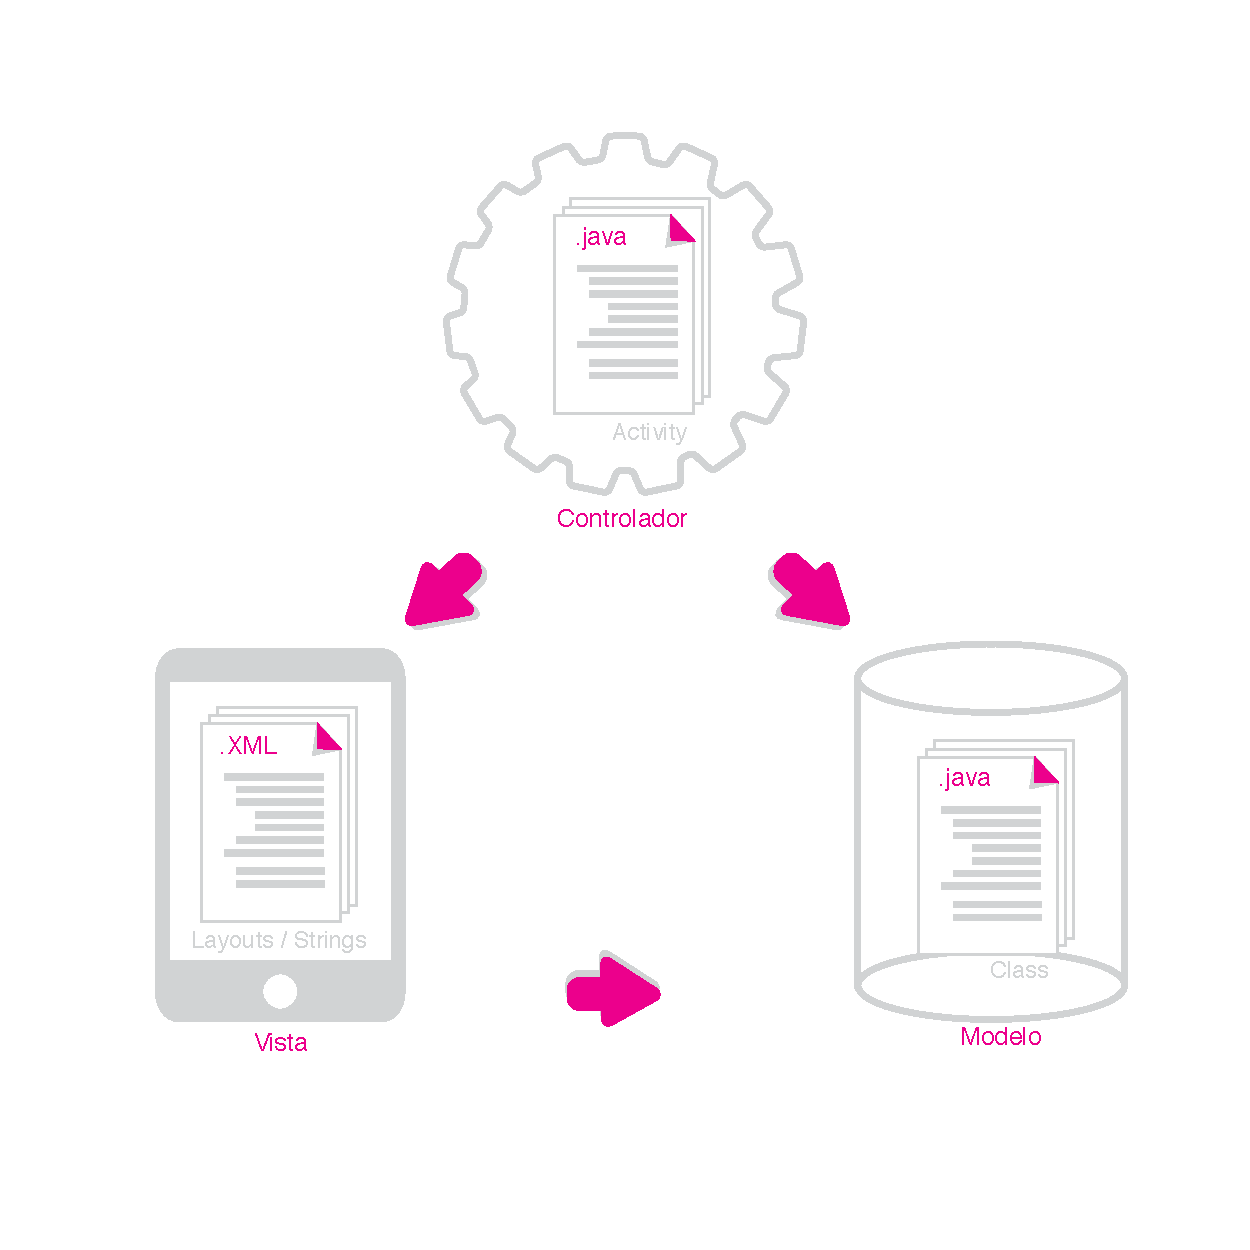
\includegraphics[scale=0.5]{./imgs/esquemas/mvc.pdf}
\caption{Generación parcial de clases}
\label{fig:mvc}
\end{figure}

En la figura \ref{fig:mvc}, vemos el esquema del patrón de desarrollo MVC aplicado en una aplicación Android.\par
Las partes de las que se compone una aplicación Android son las siguientes:
\begin{itemize}
\item \textbf{Vista}: La vista de la aplicación se desarrolla mediante ficheros XML. La vista en Android se compone fundamentalmente por dos elementos: los ficheros XML que definen la interfaz de usuario, que podemos encontrar en \emph{\textbackslash{res}\textbackslash{layout}} y por otra parte tenemos los ficheros XML con las cadenas de texto que se utilizarán en la interfaz, correctamente internacionalizadas y almacenadas en \emph{\textbackslash{res}\textbackslash{values}}. Adicionalmente se puede definir estilos para los elementos de la interfaz gráfica, análogamente a como se hace en CSS, estos ficheros de estilo los podemos encontrar también en \emph{\textbackslash{res}\textbackslash{values}}. Para soportar distintos tipos de pantalla en Android, las imágenes y los estilos se organizan dentro de carpetas determinadas en la aplicación Android y en función de la resolución del dispositivo se cargarán unas u otras.
\item \textbf{Modelo}: El modelo en para una aplicación Android no difiere del modelo en otro lenguaje. Se trata de una serie de clases con la información del sistema. En nuestro caso serán las clases que contengan la información del informe médico. Encapsularemos el modelo dentro del paquete \emph{model}.
\item \textbf{Controlador}: Finalmente los controladores en las aplicaciones Android son las Actividades (\emph{Activity}). Las actividades gestionan la interfaz de usuario, interactuan con el usuario y acceden al modelo bien para mostrarlo en la vista o para modificarlo. 
\end{itemize}

Finalizaremos este apartado viendo la estructura de ficheros de la aplicación Android que nos servirá como framework para instanciar las aplicaciones concretas sobre un informe DICOM-SR y señalando las rutas dónde irán los ficheros que generaremos.\par

\begin{figure}
\centering
\framebox[1.05\textwidth]{%
\begin{minipage}{0.95\textwidth}
	\dirtree{%
		.1 meer-framework/.
		.2 {\color{RubineRed} AndroidManifest.xml.}
		.2 assets/. 
		.3 \vdots.
		.2 bin/. 
		.3 \vdots.
		.2 gen/. 
		.3 \vdots.
		.2 libs/. 
		.3 \vdots.
		.2 src/.
		.3 com/.
		.4 i3m/.
		.5 meer/.
		.6 {\color{RubineRed} *.java }\DTcomment{\emph{Actividades}}.
		.6 model/.
		.7 {\color{RubineRed} *.java }\DTcomment{\emph{Modelo}}.
		.2 res/.
		.3 drawable-hdpi/.
		.4 \vdots\DTcomment{\emph{Iconos e imágenes para alta resolución (> 640dp x 480dp)}}.
		.3 drawable-ldpi/.
		.4 \vdots\DTcomment{\emph{Iconos e imágenes para baja resolución (> 426dp x 320dp)}}.
		.3 drawable-mdpi/.
		.4 \vdots\DTcomment{\emph{Iconos e imágenes para resolución media (> 470dp x 320dp)}}.
		.3 drawable-xhdpi/.
		.4 \vdots\DTcomment{\emph{Iconos e imágenes para extra alta resolución (> 960dp x 720dp)}}.
		.3 layout/.
		.4 {\color{RubineRed} *.xml }\DTcomment{\emph{Vista: UI}}.
		.2 menu/. 
		.3 \vdots\DTcomment{\emph{Vista: menús}}.
		.2 values/. 
		.3 {\color{RubineRed} *.xml }\DTcomment{\emph{Vista: estilos y cadenas de texto}}.
		.2 values-11/. 
		.3 {\color{RubineRed} *.xml }\DTcomment{\emph{Vista: estilos para API 11}}.
		.2 values-14/. 
		.3 {\color{RubineRed} *.xml }\DTcomment{\emph{Vista: estilos para API 14}}.
	}
\end{minipage}
}
\caption{Estructura de ficheros de la aplicación framework Android}
\end{figure}

\subsection{Aplicación generadora de código}
\subsubsection{Diagrama de clases}


\section{Diseño de interfaces}

\section{Prototipo}